\documentclass[14pt]{beamer}
\usetheme{Antibes}
\usecolortheme{lily}

\usepackage[T1]{fontenc}
\usepackage[utf8]{inputenc}
\usepackage{upgreek}
\usepackage{polski}
\usepackage[polish]{babel}
\usepackage{url}
\usepackage{listings}

\usepackage{parskip}
\newcommand{\fakehead}[1]{``\textit{#1}''}

\graphicspath{{assets/}}
\lstset{
   extendedchars=true,
   basicstyle=\footnotesize\ttfamily,
   showstringspaces=false,
   showspaces=false,
   tabsize=2,
   breaklines=true,
   showtabs=false,
   captionpos=b
}

\author{Antoni Mleczko, Maciej Mionskowski}
\title[BSGenerator]{\Huge{B{\tiny{ull}}S{\tiny{hit}} Generator}}
\date{Rok Akademicki 2018/2019---IV semestr}
\subtitle{\small{\fakehead{Co zaprezentowali kandydaci nie wytrzymujący morderczej pracy w amazonie?}}}

\institute{Wydział Informatyki, Elektroniki i Telekomunikacji}

\setcounter{tocdepth}{1}

\begin{document}

\begin{frame}
\titlepage
\end{frame}

\begin{frame}{Agenda}{\fakehead{Wstęp do zbrodni warunkiem dobrych relacji.}}
\tableofcontents
\end{frame}

\begin{section}{Cele}
	\begin{frame}{Cele}{\fakehead{Klatka schodowa do\underline{cel}owo zaprasza na dobry humor.}}
		\begin{enumerate}
			\item Generacja zrozumiałych artykułów i nagłówków
			\item Zrównoleglony, rozproszony web scraper
			\item Heurystyczna ekstrakcja ciała artykułów ze stron internetowych
		\end{enumerate}
	\end{frame}
\end{section}

\begin{section}{Scraper}
	\begin{frame}{Scraper}
	\end{frame}
\end{section}

\begin{section}{Content Extractor}
	\begin{frame}{Ekstrakcja ciała}{\fakehead{Artykuły są głupie, durne i absurdalne}}
			%{\fakehead{Sukces polskiej policji, zobacz jak rozpoznać ruskiego trolla w internecie, pobierz bezpłatny (?)}}
		\centering
		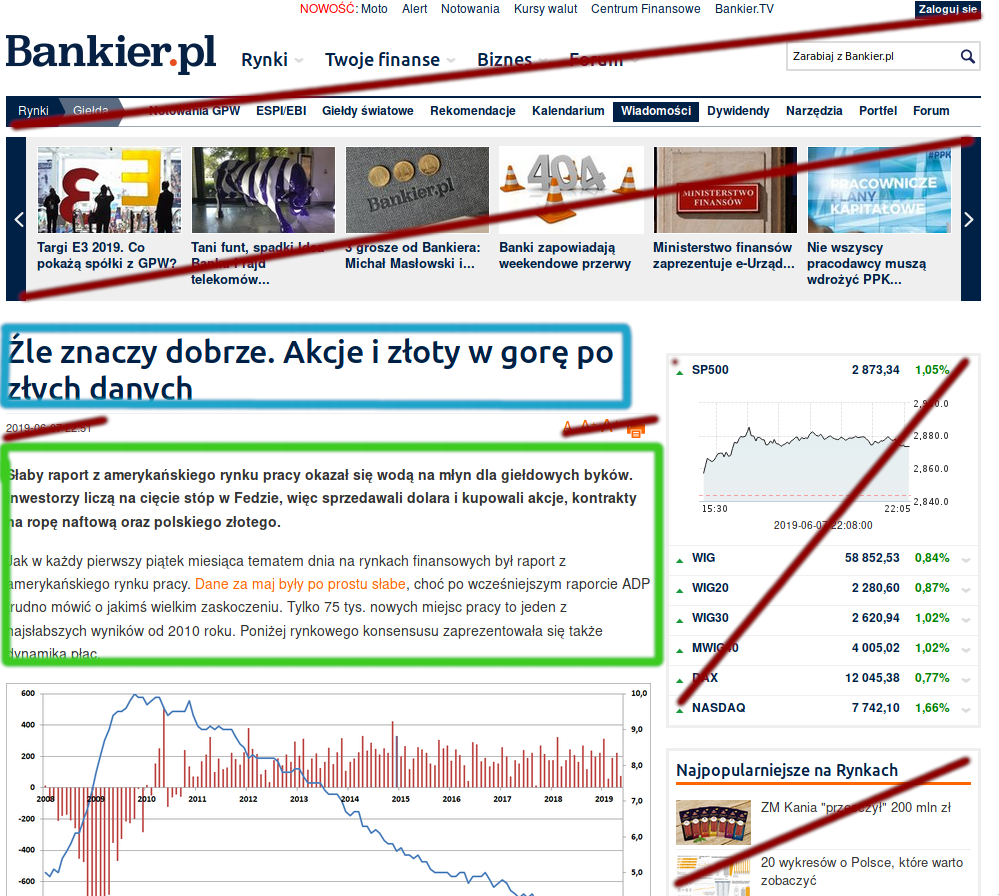
\includegraphics[width=0.6\linewidth]{bankier.png}
	\end{frame}
	\subsection{Header}
	\begin{frame}[fragile]{Tytuł}{\fakehead{Tytuł w Fakcie - redaktor naczelny przeprasza, dziennikarze umywają ręce papieża Franciszka.}}
	\begin{lstlisting}
<meta property="og:title" content="Zle znaczy dobrze. Akcje i zloty w gore po zlych danych">

<title>Zle znaczy dobrze. Akcje i zloty w gore po zlych danych - Bankier.pl</title>
	\end{lstlisting}
	\end{frame}
	\subsection{Content}
	\begin{frame}[fragile]{Treść}{\fakehead{Rzyganie w tramwaju - jest wielu rannych i zabitych dzieci}}

		\begin{enumerate}
			\item System punktacji dla elementów na stronie
			\item Liczba przecinków w blokach tekstu
				%\begin{enumerate}
				%	\item{Łączenie bloków tekstu na jednym poziomie w jeden}
				%	\item{Łączenie bloków tekstu wertykalnie w jeden z mniejszą punktacją}
				%\end{enumerate}
			\item Długość tekstu
			\item Filtracja elementów po zahardcodowanych klasach css
		\end{enumerate}
	\end{frame}
\end{section}

\begin{section}{Data Set}
	\begin{frame}{Data Set}
	\end{frame}
\end{section}

\begin{section}{Generator}
	\subsection{LSTM}

	\begin{frame}{LSTM}
		Long-short-term memory, recurrent neural network.
		\begin{enumerate}
			\item Finalna implementacja: Deeplearning4j, prototyp: Python (Keras)
			\item Sieć neuronowa oparta na znakach
			\item 3 warstwowa architektura
			\item 580 000 parametrów
		\end{enumerate}
	\end{frame}
	\begin{frame}[fragile]{LSTM}
		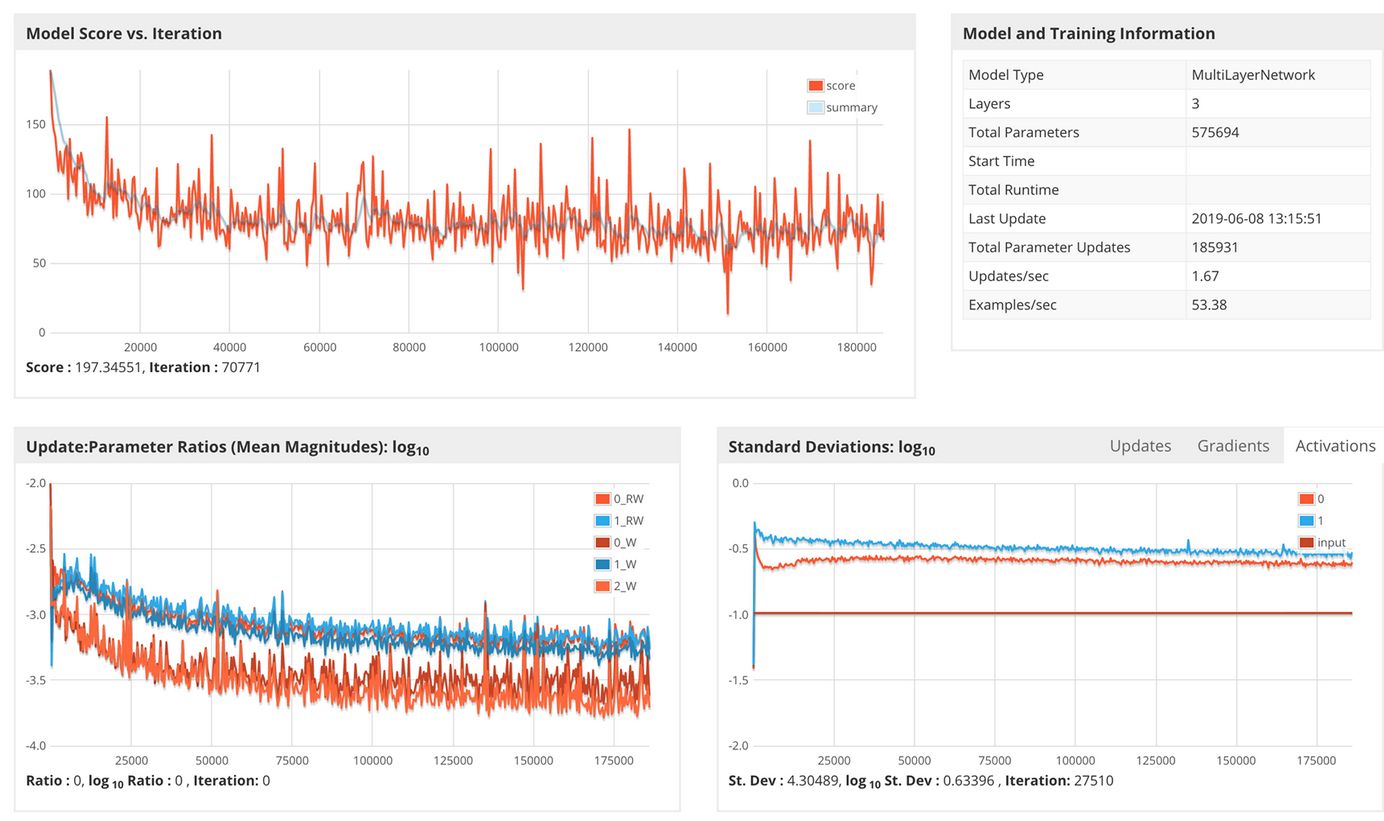
\includegraphics[width=\linewidth]{lstm.png}
	\end{frame}
	\begin{frame}{Wyniki}{\fakehead{Nie udało się zrealizować w kolejnej rundzie australian open}}
			{\textit{\_"iorjwein weopr12 śćfre234}}
		\begin{enumerate}
			\item Ściana obliczeniowa i czasowa
			\item Problemy z CUDA, CUDART, CUDnn
			\item Dataset średniej jakości
		\end{enumerate}
	\end{frame}
	\subsection{Markov}
	\begin{frame}{Markov Chain}{\fakehead{Ogniwo niewidzialnego łańcucha spajającego polskość oznacza solidarność, wolność, wielkość narodu polskiego}}
		\centering
		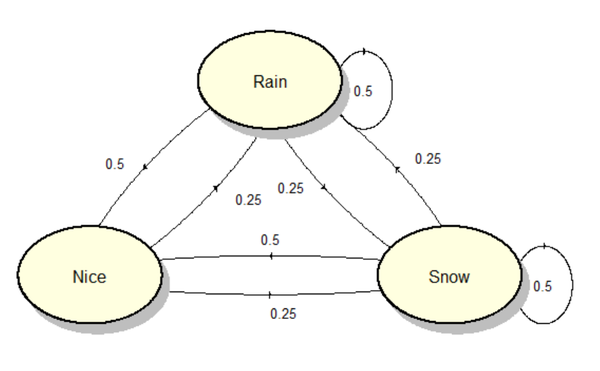
\includegraphics[width=0.8\linewidth]{markov.png}
	\end{frame}
	\begin{frame}{n-grams}{\fakehead{Ile waży dusza? 21 gramów.}}
		\centering
		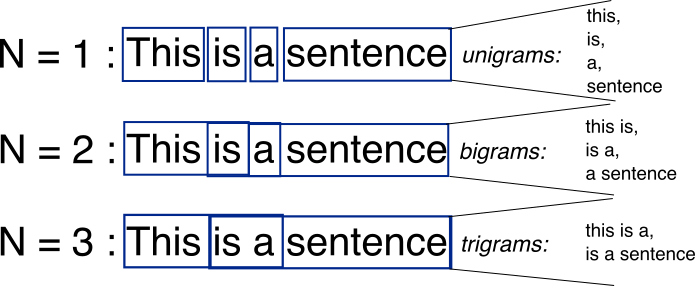
\includegraphics[width=0.8\linewidth]{ngrams.png}
	\end{frame}
	\begin{frame}{Wyniki}{\fakehead{Wyniki kontroli escape roomu w koszalinie, marsz równości jednak przejdzie}
			}
		\begin{enumerate}
			\item w miami miałem spotkania a między spotkaniami pochodziłem po wodzie w kranie 
			\item sodą oczyszczoną ratuje maturzystów broniarz kręci nosem
			\item pigułka odbiera kobiecie ochotę na mielone w surowej szynce parmeńskiej z jajkiem  
			\item seksistowski horror w uk zabito nawet 4700 dziewczynek ze względu na ciężar historii pomiędzy niemcami a rosją 
		\end{enumerate}
	\end{frame}
\end{section}

\begin{section}{Pytania}
	\begin{frame}{Pytania}{\fakehead{Efekt franciszka - coraz więcej pytań niż odpowiedzi}}
		\centering
		
\includegraphics[width=0.5\linewidth]{question.png}
	\end{frame}
\end{section}


\end{document}
